\hypertarget{_overview_LockerinThreadSafety}{}\section{Locker in Thread Safety}\label{_overview_LockerinThreadSafety}
In the context of multi-\/threaded programs, shared data and be read and written by multiple threads during simultaneous execution. To keep the data correct, usually a locker is required. The function of locker is to make data to be accessed by only one thread at any given time. For example, one thread tries to update the data. It locks the data to make it inaccessible by any other threads. After change, it can unlock the data and now the data is available for all threads. The disadvantage of locker is if one thread need to access the data but the data is locked by another thread, it should wait until the data is unlocked. ~\newline
~\newline
\label{_overview_eg1}%
\hypertarget{_overview_eg1}{}%
Example 1 
\begin{DoxyImageNoCaption}
  \mbox{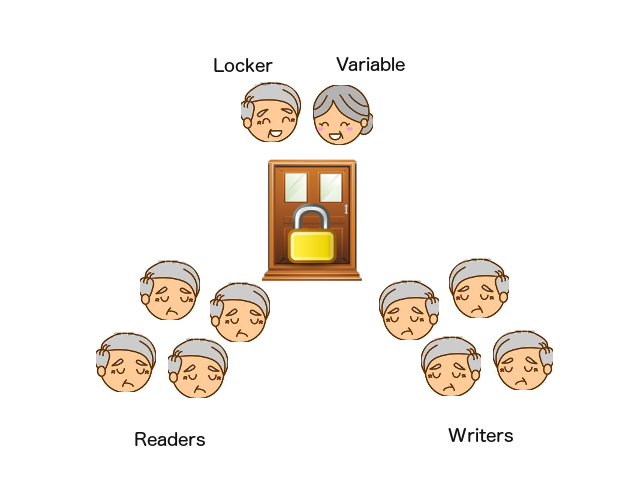
\includegraphics[width=\textwidth,height=\textheight/2,keepaspectratio=true]{ResearchOverviewLockerinThreadSafety.png}}
\end{DoxyImageNoCaption}

\begin{DoxyItemize}
\item A variable is locked by a thread
\item 100 threads need to read the variable
\item 100 threads need to write the variable
\end{DoxyItemize}

In this case, 200 threads are waiting for one variable.\hypertarget{_overview_Theideaofthisproject}{}\section{The idea of this project}\label{_overview_Theideaofthisproject}
The idea of this project is to make the variable in to two states\+: one for read and the other one for write. This is why the project name is Dual State Framework. Any time, a thread tries to lock the variable will lock the write copy. The read copy is always available for all thread. It means only threads that try to write the variable need wait. Back to \hyperlink{_overview_eg1}{Example 1}, now we have only 100 threads are waiting. 
\begin{DoxyImageNoCaption}
  \mbox{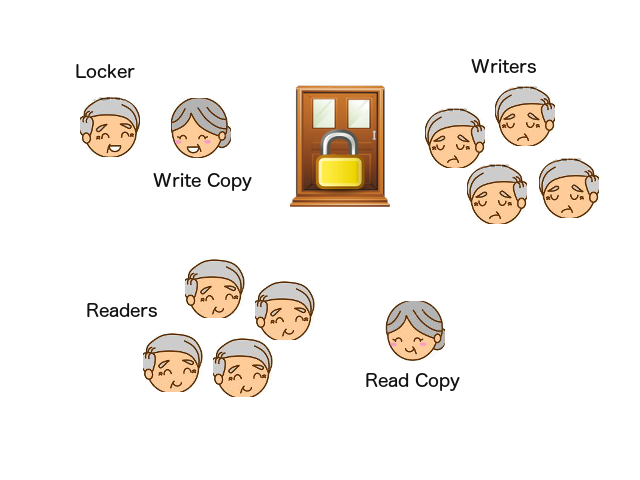
\includegraphics[width=\textwidth,height=\textheight/2,keepaspectratio=true]{ResearchOverviewTheideaofthisproject.png}}
\end{DoxyImageNoCaption}
 